\definecolor{singleShotColor}{RGB}{196,106,28}
\definecolor{pipelineColor}{RGB}{44,138,100}
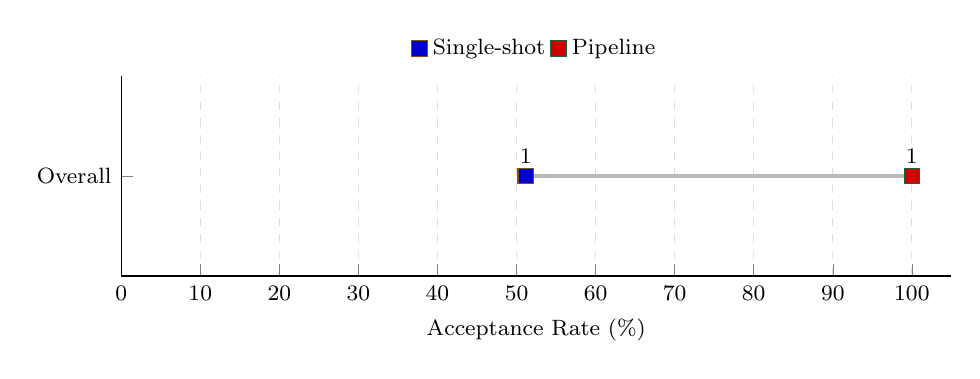
\begin{tikzpicture}
\begin{axis}[
    width=\columnwidth,
    height=0.34\columnwidth,
    xmin=0,
    xmax=105,
    ymin=0.4,
    ymax=1.6,
    xlabel={Acceptance Rate (\%)},
    ytick={1},
    yticklabels={Overall},
    axis lines*=left,
    xmajorgrids=true,
    grid style={dashed,gray!25},
    tick label style={font=\footnotesize},
    label style={font=\footnotesize},
    legend style={
        draw=none,
        font=\footnotesize,
        at={(0.5,1.03)},
        anchor=south,
        legend columns=2
    }
]
\addplot+[very thick,gray!55,mark=none,forget plot] coordinates {(51.16,1) (100.00,1)};

\addplot+[
    only marks,
    mark=square*,
    mark size=2.8pt,
    fill=singleShotColor,
    draw=singleShotColor!70!black,
    nodes near coords,
    nodes near coords style={font=\footnotesize, text=black, anchor=south, yshift=1pt},
] coordinates {(51.16,1)};

\addplot+[
    only marks,
    mark=square*,
    mark size=2.8pt,
    fill=pipelineColor,
    draw=pipelineColor!70!black,
    nodes near coords,
    nodes near coords style={font=\footnotesize, text=black, anchor=south, yshift=1pt},
] coordinates {(100.00,1)};

\legend{Single-shot,Pipeline}
\end{axis}
\end{tikzpicture}
